        %auto-ignore
\section{Introduction}

Deep neural networks have showcased remarkable performance across a broad range of tasks, including image classification, game playing exemplified by AlphaGo \citep{alphago}, and natural language processing demonstrated by GPT-4 \citep{openai2023gpt4}. A prevailing trend in developing these networks is to increase their size and complexity, with empirical evidence indicating that using the same computation resources, models with more parameters tend to exhibit better performance. There are two ways to increase any network size: \emph{width} and \emph{depth}. The properties of the width (given a fixed depth) have been extensively studied in the literature: recent work by \citet{yang2022tensor} identified the \emph{Maximal Update Parametrization} ($\mu$P) that guarantees maximal feature learning in the infinite width limit.\footnote{Here maximal feature learning refers to $\Theta(1)$ change in features in the infinite width limit. This should be contrasted with the lazy training regime where the change in features is of order $\Theta(n^{-1/2})$.} Another benefit of $\mu$P is hyperparameter transfer which enables hyperparameter tuning on smaller models; the optimal hyperparameter choice for the smaller model remains optimal for larger models (i.e., models with larger width). However, despite the achievements of large-scale deep models and the theoretical understanding of scaling width, increasing the depth of neural networks still has both practical limitations and theoretical difficulties. In practice, increasing depth beyond some level often results in performance degradation and/or significant shifts in the optimal hyperparameters. In theory, unlike increasing width, increasing depth introduces new parameters that significantly change the training dynamics. In this paper, we aim to solve this problem by extending $\mu$P to include depth scaling. We call the depth scaling Depth-$\mu$P.

The issue of depth scaling has persisted over time. A decade ago, deep neural networks experienced significant degradation problems --- having more than a few dozen layers would increase the training error instead of improving the model's performance. This was partly due to the vanishing or exploding gradient problem that affects the efficient propagation of information through the network. The introduction of residual networks (ResNet)~\citep{he2016deep,he2016identity, srivastava2015highway} has partially resolved this issue, allowing for the training of deeper networks with improved performance. ResNet is constructed by layering \emph{residual blocks}, which are composed of a series of convolutional layers and then an element-wise addition with the input. This element-wise addition (commonly referred to as \emph{skip connection}) is a significant innovation of ResNet and remains an important ingredient in modern architectures including Transformers \citep{vaswani2017attention}. 

Specifically, in a residual architecture, the $l$-th residual block is formulated as
\[x^l=x^{l-1} + g^l(x^{l-1};W^l),\] 
where $x^{l-1}$ is the input, $x^l$ is the output, $W^l$ are the parameters of the block, and $g^l$ (often called the \emph{residual branch}) is a mapping that defines the layer (e.g. a stack of convolutions in ResNet, or SelfAttention and MLP in a Transformer). In this work, we focus on the case where $g^l$ is a biasless perceptron with (or without) activation.

\begin{table}[t]
\begin{center}
\caption{Difference between standard depth scaling and Depth-$\mu$P. The constants $a$ and $\eta$ in Depth-$\mu$P are transferable across depth, i.e., one can tune a smaller network and use the same constants for deeper networks. On the other hand, the learning rate of standard depth scaling requires separate tuning for models of different depth. }
\begin{tabular}{c c c c} 
 \hline
  & Branch Multiplier & Learning Rate  \\
 \hline
 \vspace{-0.7em}
 \\
 Standard & 1 & ? (tuned) \\ 

 Depth-$\mu$P (SGD) & {\color{Maroon} $a/\sqrt{\textrm{depth}}$} & {\color{Maroon} $\eta$} \\ 

 Depth-$\mu$P (Adam) & {\color{Maroon} $a/\sqrt{\textrm{depth}}$} & {\color{Maroon} $\eta/\sqrt{\textrm{depth}}$}  \\
\hline

\end{tabular}
\end{center}
\end{table}

The stacking of many residual blocks causes an obvious issue even at the initialization --- the norm of $x^l$ grows with $l$, so the last layer features do not have a stable norm when increasing the depth. Intuitively, one can stabilize these features by scaling the residual branches with a depth-dependent constant. However, scaling the residual branches with arbitrarily small constants might result in no feature learning in the large depth limit since the gradients will also be multiplied with the scaling factor. 

When each block $g^l$ has only one layer (one matrix multiply), we identify the parametrization we call Depth-$\mu$P as the optimal parametrization for deep networks.
It maximizes both \emph{feature learning} and \emph{feature diversity}\footnote{We give a formal definition of feature learning and feature diversity later in the paper.}  among all possible parametrizations of block multiplier and learning rate with depth.
Our framework extends the previous results on $\mu$P which deals with optimal width scaling \citep{yang2022tensor}. It completes the width scaling and hence provides a full width and depth scaling recipe that guarantees maximal feature learning and hyperparameter transfer across width and depth.  %
Depth-$\mu$P contains the following modifications to the standard practice:

\begin{enumerate}
    \item There is a multiplier for each residual branch before adding to its input, which is inversely proportional to the square root of $L$ (where $L$ is the depth). Formally, with a constant $a$ independent from $L$,
    \begin{align}
        x^{l}&=x^{l-1} +\frac a {\sqrt L} \cdot g^l(x^{l-1}; W^l). \label{eqn:resmlp_defn}
    \end{align}
    \item We set the learning rate of $W^l$ so that the update of $W^l$ during training is proportional to $1/\sqrt L$. We derive different learning rate schemes for different optimization algorithms based on this principle. For Adam, because it is scale-invariant to the gradient, the learning rate of $W^l$ is set to be $\eta/{\sqrt{L}}$. On the other hand, the learning rate of $W^l$ for SGD is set as a constant $\eta$ because the gradient of $W^l$ is already of size $1/\sqrt{L}$ due to the multiplier.
\end{enumerate}
In block depth $1$ (i.e., $g^{l}$ is a biasless perceptron, $W^{l}$ is a single matrix), this scaling leads to the following properties:
\begin{itemize}
    \item At the initialization, each one of the $L$ residual blocks contributes $\Theta(1/\sqrt L)$ to the main branch. These $L$ contributions are independent of each other, so the sum of them is of size $\Theta(1)$.
    \item During training, the contribution of the update of each residual block is $\Theta(1/L)$ due to the combining effect of the learning rate and multiplier. The contributions of the updates are highly correlated, so they sum up to $\Theta(1)$.
\end{itemize}
More detailed intuition of this scaling approach can be found in \Cref{sec:intuition} where we provide a simple analysis with linear networks after one gradient step. We give a complete classification of depthwise parametrizations in \cref{sec:convergence}.

\begin{wrapfigure}{r}{0.5\textwidth}
  \vspace{-1cm}
    \centering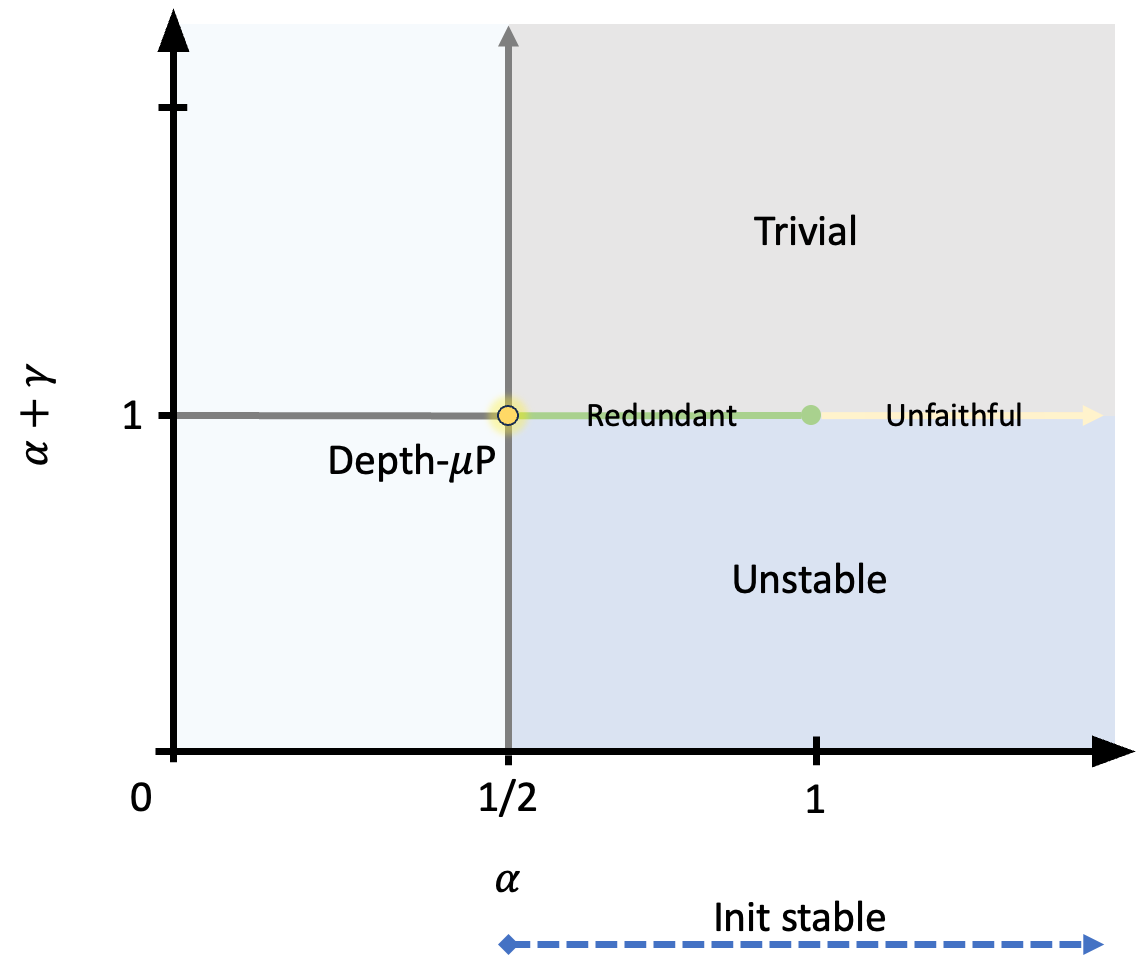
\includegraphics[width=0.5\textwidth]{fig/bd1_phase_diagram.png}
  \caption{Behaviors of scaling strategies with a branch multiplier $L^{-\alpha}$ and parameter update proportional to $L^{-\gamma}$. }
  \label{fig:alpha-gamma}
  \vspace{-1cm}
\end{wrapfigure}
\subsection{Optimality of Depth-$\mu$P. } 

We thoroughly compare Depth-$\mu$P with other scaling strategies with a branch multiplier $\propto L^{-\alpha}$ and parameter update  $\propto L^{-\gamma}$.\footnote{It implies that the effective learning rate is proportional to $L^{-\gamma}$ for Adam and $L^{\alpha-\gamma}$ for SGD if the network is stable at initialization.}  As shown in \Cref{fig:alpha-gamma}, the space of $(\alpha, \gamma)$ is divided into several areas, each resulting in a different behavior when $L\to \infty$: 
\begin{itemize}[leftmargin=*]
    \item Having $\alpha\geq 1/2$ is required to stabilize the network at initialization. This ensures that he hidden activations and the network output do not explode at initialization;
    \item For any $\alpha+\gamma < 1$, the network is unstable during training. The change in hidden activations or the network output explodes with depth during training;
    \item For any $\alpha+\gamma > 1$, training outcome is trivial. The change of the network vanishes as depth increases;
\end{itemize}

\begin{itemize}[leftmargin=*]
    \item For any $\alpha+\gamma=1$ with $\alpha > 1$, the network is \emph{unfaithful} (a formal definition will provided later in the paper). The hidden activations explode during training as depth increases;
    \item For any $\alpha + \gamma = 1$ and $\alpha \in (1/2, 1]$, we show that the network converges to a \emph{redundant} limit that lacks \emph{feature diversity}, in that close layers have similar outputs (in a neural ODE fashion). 
    \item The only choice of $\alpha$ and $\gamma$ left is $\alpha = \gamma = 1/2$, which corresponds to Depth-$\mu$P.
\end{itemize}
The rigorous definitions and proofs are presented in \Cref{sec:convergence}. 

\subsection{Hyperparameter Transfer for Depth.} 
The optimality of Depth-$\mu$P implies (under some assumptions) that the optimal hyperparameters of the networks also converge as the depth ($L$) increases.
This convergence suggests that the optimal hyperparameters of shallower networks are approximately equal to those of deeper networks. As a direct implication, we can leverage this property to infer the hyperparameters for deeper networks from the shallower ones, effectively reducing the cost associated with hyperparameter tuning. With Depth-$\mu$P, we successfully train networks comprising thousands of residual blocks, while also showcasing the transferability of hyperparameters across depth.

\subsection{Impossibility Results for Block Depth $\ge 2$}

While the block depth 1 case admits a positive result, we show that the block depth $\ge 2$ case does not and cannot (\cref{sec:bd2}). The basic issue is the weights in different layers within a block is forced to interact additively instead of multiplicatively when depth is large, if one wants to retain diversity.
This causes block depth $\ge 2$ to have worse performance than block depth $1$ and for the optimal hyperparameters to shift with depth.
We demonstrate this pedagogically on resnet with MLP blocks but also on Megatron transformer~\citep{shoeybi2019megatron} trained on Common Crawl.
These observations entail the need to rethink the current approach to hyperparameter transfer.

